\documentclass{article}
\usepackage[a4paper]{geometry}
\usepackage{bookmark}
\usepackage{amsmath,amsfonts,amsthm,amssymb,mathtools}
\usepackage[italian]{babel}
\usepackage{graphicx}
\title{\Huge{Pendolo fisico}}
\author{\huge{Giosué Aiello, Domenico Fenili, Francesco Sermi}}
\date{14 Novembre 2023}

\begin{document}

\maketitle
\pagebreak
\tableofcontents
\pagebreak

\section{Scopo dell'esperienza}
Lo scopo di questa esperienza è quello di misurare il periodo di un pendolo fisico in funzione della distanza del perno di rotazione dal centro di massa.

\section{Cenni teorici}

\begin{figure}[h!]
	\centering
	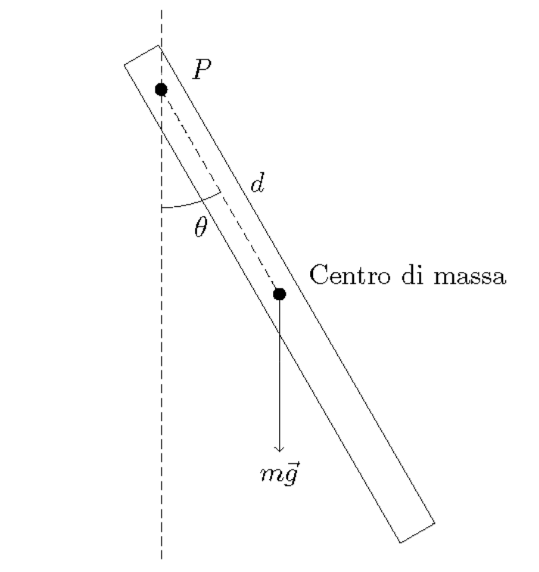
\includegraphics[scale=0.35]{pendolo_fisico.png}
	\caption{Immagine schema del nostro apparato sperimentale}
	\label{fig:schema_pendolo}
\end{figure}
Un oggetto fissato ad un punto di sospensione $P$ (che dista $d$ dal centro di massa) e soggetto alla gravità costituisce un pendolo fisico. Se questo corpo viene spostato di un angolo $\theta$ dalla sua posizione di equilibrio, il momento torcente della forza di gravità (rispetto al punto di sospensione $P$) vale:
\begin{equation*}
	\tau = -mgd\sin{\theta}
\end{equation*}
che, per $\theta << 10^\circ - 15^\circ$ possiamo esprimere $sin(\theta)$ utilizzando la formula di espansione in serie di Taylor al primo ordine:
\begin{equation*}
	\sin{\theta} \approx \theta + o(\theta^3)
\end{equation*}
Pertanto possiamo riscrivere il momento torcente della forza di gravità come:
\begin{equation*}
	\tau = -mgd\theta
\end{equation*}
E per la seconda equazione cardinale si ha che:
$$
	\tau = \frac{dL}{dt}
$$
e sapendo che il momento angolare di un pendolo fisico risulta essere pari a $L = I\omega$ e $\omega = \frac{d\theta}{dt}$ si ha che:
$$
	\tau = \frac{dL}{dt} = I\frac{d}{dt} \left(\frac{d\theta}{dt} \right) = I\frac{d^2 \theta}{dt^2}
$$
ne segue immediatamente che:
$$
	I\frac{d^2 \theta}{dt^2} = -mgd\theta \implies \frac{d^2 \theta}{dt^2} + \frac{mgd}{I}\theta = 0 
$$
Siamo dinanzi ad un'equazione differenziale di secondo ordine a coefficienti costanti omogenea e in questo caso è l'equazione differenziale di un moto armonico. Ponendo $-\omega_0^2 = -\frac{mgd}{I}$: 
$$\omega_0 = \sqrt{\frac{mgd}{I}} \implies T_0 = 2\pi\sqrt{\frac{I}{mgd}}$$
Utilizzando il teorema degli assi paralleli, possiamo concludere che il momento di inerzia dell'oggetto fisico risulta essere:
$$
	I = I_{cm} + md^2 = \frac{ml^2}{12} + md^2
$$
Possiamo quindi riscrivere la formula nella seguente maniera:
$$
	T(d) = \sqrt{\frac{m(l^2 + d^2)}{mgd}} = \sqrt{\frac{\frac{l^2}{12} + d^2}{gd}}
$$

\end{document}
